% ------------------------------------------------------------------------------
% TYPO3 Version 10.4 - What's New (Dutch Version)
%
% @license	Creative Commons BY-NC-SA 3.0
% @link		https://typo3.org/help/documentation/whats-new/
% @language	Dutch
% ------------------------------------------------------------------------------

\section{Wijzigingen voor integrators}
\begin{frame}[fragile]
	\frametitle{Wijzigingen voor integrators}

	\begin{center}\huge{Hoofdstuk 2:}\end{center}
	\begin{center}\huge{\color{typo3darkgrey}\textbf{Wijzigingen voor integrators}}\end{center}

\end{frame}

% ------------------------------------------------------------------------------
% Feature | 89513 | Provide password recovery for backend users

\begin{frame}[fragile]
	\frametitle{Wijzigingen voor integrators}
	\framesubtitle{Wachtwoord herstellen e-mail (1)}

	\begin{itemize}

		\item Herstellen van wachtwoorden voor backend-gebruikers zijn maar 4 uur geldig.\newline
			Deze tijdslimiet is niet aanpasbaar.
		\item Voor betere beveiliging kan de functie uitgeschakeld worden voor admin-gebruikers of alle gebruikers.
		\item Als gebruikers hetzelfde e-mailadres hebben wordt een andere tekst gebruikt in de mail.
		\item TCA-veld \texttt{be\_users.email} mag niet ingesteld zijn op \texttt{eval=email}.

		\item De functie werkt alleen voor gebruikers, die:
			\begin{itemize}
				\item een e-mailadres ingesteld hebben,
				\item een wachtwoord ingesteld hebben en
				\item niet uitgeschakeld/verwijderd zijn.
			\end{itemize}

	\end{itemize}

\end{frame}

% ------------------------------------------------------------------------------
% Feature | 89513 | Provide password recovery for backend users

\begin{frame}[fragile]
	\frametitle{Wijzigingen voor integrators}
	\framesubtitle{Wachtwoord herstellen e-mail (2)}

	\begin{itemize}
		\item E-mails voor herstellen van wachtwoorden kunnen ook via de commandoregel verstuurd worden.
	\end{itemize}

	\begin{figure}
		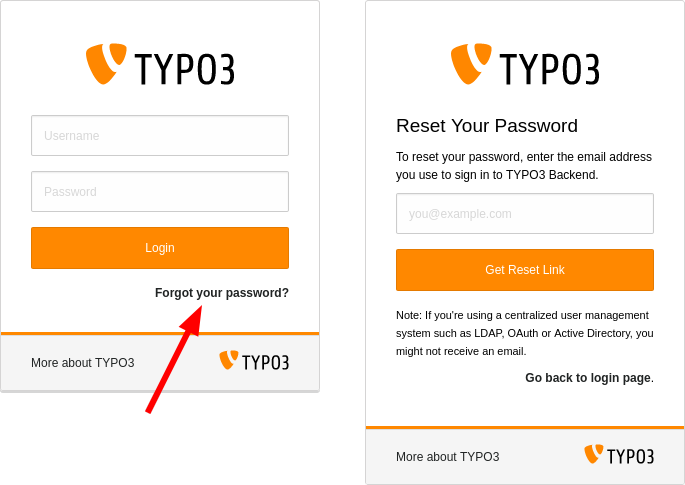
\includegraphics[width=0.9\linewidth]{ChangesForIntegrators/89513-ProvidePasswordRecoveryForBackendUsers.png}
	\end{figure}

\end{frame}

% ------------------------------------------------------------------------------
% Important | 90285 | Fresh installs without constraint for typo3fluid/fluid will get version 3.0+

\begin{frame}[fragile]
	\frametitle{Wijzigingen voor integrators}
	\framesubtitle{Fluid Templating Engine}

	\begin{itemize}
		\item De TYPO3 core is volledig compatibel met Fluid versies 2.6+ en 3.0+
		\item Nieuwe installaties zonder afhankelijkheid zullen Fluid versie 3.x gebruiken
			(\texttt{typo3fluid/fluid:\^{}3}).
		\item Als het project Fluid sjablonen bevat die niet werken met versie 3.0+ neem dan
			een van de volgende stappen:

			\begin{itemize}
				\item Beperk de maximale versie: \texttt{typo3fluid/fluid:\^{}2}
				\item Werk Fluid sjabolen bij.
			\end{itemize}

	\end{itemize}

\end{frame}

% ------------------------------------------------------------------------------
% Important | 18079 | pages.doktype restriction for frontend queries refined

\begin{frame}[fragile]
	\frametitle{Wijzigingen voor integrators}
	\framesubtitle{Paginatype afhandeling}

	\begin{itemize}
		\item Interne afhandeling van paginatypes is gewijzigd.
		\item De optie \texttt{pages.doktype} bepaalt een getal dat het type voorstelt,
			bijv. standaardpagina, map, snelkoppeling, link naar externe URL, enz.
		\item Pagina's van een bepaald type (bijv. map en prullenbak) waren uitgezonderd als inhoud
			werd gelezen uit een specifieke pagina of als records werden uitgelezen.
		\item De beperking is verwijderd en eigen paginatypes met een getal >200 zijn nu mogelijk.
		\item Integrators en ontwikkelaars die pagina doktypes hebben gebruikt, bijv. in TypoScript,
			wordt aangeraden te kijken of het oude gedrag werd misbruikt en nu bijgewerkt moet worden.
	\end{itemize}

\end{frame}

% ------------------------------------------------------------------------------
% Feature | 90826 | Compare backend usergroups

\begin{frame}[fragile]
	\frametitle{Wijzigingen voor integrators}
	\framesubtitle{Module backendgebruikers}

	\begin{itemize}
		\item Integrators kunnen nu gebruikersgroepen vergelijken.
	\end{itemize}

	\begin{figure}
		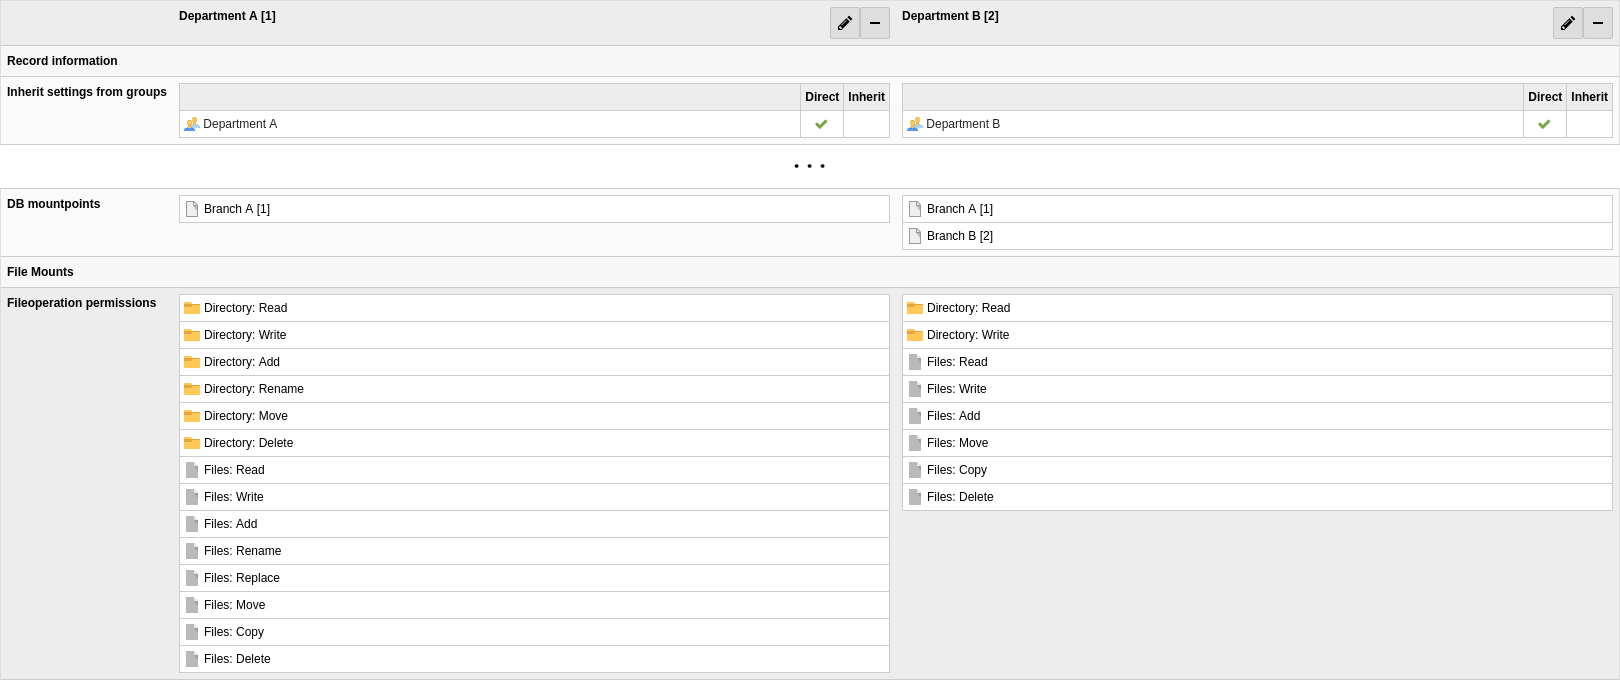
\includegraphics[width=0.9\linewidth]{ChangesForIntegrators/90826-CompareBackendUsergroups.png}
	\end{figure}

\end{frame}

% ------------------------------------------------------------------------------
% Important | 89555 | Workspace-related database records contain the proper Page ID

\begin{frame}[fragile]
	\frametitle{Wijzigingen voor integrators}
	\framesubtitle{Werkruimtes}

	\begin{itemize}
		\item Lange tijd gebruikte TYPO3 \texttt{pid} waarde \texttt{-1} voor ongepubliceerde records.
		\item TYPO3 bekijkt nu de volgende drie velden voor records in versiebeheer:

			\begin{itemize}
				\item \texttt{t3ver\_wsid} (ID van werkruimte waarin record zit)
				\item \texttt{t3ver\_state} (type van record in versiebeheer)
				\item \texttt{t3ver\_oid} (live-versie van een record)
			\end{itemize}

		\item Daarom is \texttt{pid=-1} niet meer vereist.
		\item De Upgrade Wizard zet alle \texttt{pid} velden om van records in versiebeheer
			naar de echte \texttt{pid} waarden.
		\item Nieuwe installaties hebben geen last van deze wijziging.

	\end{itemize}

\end{frame}

% ------------------------------------------------------------------------------
% Deprecation | 91030 | Runtime-Activated Packages

\begin{frame}[fragile]
	\frametitle{Wijzigingen voor integrators}
	\framesubtitle{Runtime-geactiveerd extensies}

	\begin{itemize}
		\item De volgende globale configuratie-optie is als \textbf{verouderd} aangemerkt:\newline
			\smaller
				\texttt{\$GLOBALS['TYPO3\_CONF\_VARS']['EXT']['runtimeActivatedPackages']}
			\normalsize
		\item Het gebruik van runtime-geactiveerde exensies vertraagt het systeem significant.
		\item Integrators wordt aangeraden om de nodige stappen te nemen als dergelijke waarschuwingen
			verschijnen in de verouderingslog:\newline
			\begingroup
				\fontsize{8}{10}
				\texttt{Support for runtime activated packages will be removed in TYPO3 v11.0.}
			\endgroup

	\end{itemize}

\end{frame}

% ------------------------------------------------------------------------------
